% !TeX spellcheck = es_ES
\documentclass[12pt, letterpaper]{article}

\setlength{\parskip}{\baselineskip}

\usepackage[T1]{fontenc}

\emergencystretch=1em

\usepackage[pass, letterpaper]{geometry}

\usepackage{polyglossia}
\setdefaultlanguage{spanish}

\usepackage{graphicx}

\usepackage{csquotes}

\usepackage{caption}
\usepackage{subcaption}

\usepackage{fullpage}


\usepackage{fontspec}
\setmainfont{arial}

\usepackage[style=apa, backend=biber]{biblatex}
\addbibresource{Trabajo_Bibliografico_Entrega_2.bib}
\usepackage{hyperref}
\usepackage{cleveref}
\graphicspath{{img/}}
\SetCiteCommand{\parencite}
\begin{document}

\begin{titlepage}
	\begin{picture}(400, 75)
	   \put(-40,15){
\includegraphics[width=2.3cm]{LogoUC_COLOR_.jpg}}
	   \put(30,50){PONTIFICIA UNIVERSIDAD CATOLICA DE CHILE}
	   \put(30,35){FACULTAD DE BIOLOGIA}
	   \put(30,20){Biología de la Célula - BIO141C}
	
	\end{picture}
	
	\vspace{2cm}
	\begin{center}
		
		\textbf{{\large Trabajo Bibliográfico - Entrega 2:}\\
		\vspace{1em}
		{\Large Aplicación del machine learning a la predicción del Cáncer}\\}
		
		\vspace{2.0cm}
		
		{\Large by}
		
		
		\begin{description}
			\centering
			\item {\textit{Nicol\'as Buzeta}}
			\item {\textit{Jos\'e Caceres}}
			\item {\textit{Benjamin Barrios}}
			\item {\textit{Carlos \'Alvarez}}
		\end{description}
		
		\vspace{0.5cm}
		\begin{normalsize}
			\begin{tabular}{rcl}
				\emph{Profesora} &:& Alicia Nogueras\\
				\emph{Tutor} &:& Andr\'es Carreño\\
			\end{tabular}
		\end{normalsize}
		
		\vspace{1cm}
		
		\today
		
	\end{center}
\end{titlepage}

\newpage

\tableofcontents

\newpage

\section{Introducción}

Sabemos que dentro de las células que existen en nuestro organismo hay un núcleo (células procariontes), y este núcleo tiene en su interior una organización espacial característica, la cual a su vez depende de la matriz nuclear como de la lámina nuclear. La matriz nuclear es una red de fibras que se encuentra distribuida en todo el interior de los núcleos celulares y, además de dar rigidez al núcleo, mantiene el orden en su interior. Por otro lado, la lámina nuclear es una red que al igual que la matriz, da rigidez al núcleo, pero también regula eventos como la replicación de ADN y la división celular \autocite[p.~200]{albertsBiologiaMolecularCelula2010, zinkNuclearStructureCancer2004}. En células cancerígenas, ambas de estas estructuras se pueden ver afectadas. Esto comúnmente se refleja en un cambio morfológico del núcleo, que va de un aspecto elipsoidal a uno irregular. 


La estructura del núcleo final en estas células malignas posee diferencias características en la arquitectura nuclear con una célula sana o incluso entre esas mismas células cancerígenas hay diferencias especiales. \autocite{rynearsonNuclearStructureOrganization2011}. Esto conlleva la posibilidad de detectar células cancerígenas por su forma, y más aún, identificar el tipo de cancer en específico. Así, poder detectar estos cambios no solo ayudaría a encontrar el cáncer, sino también a detectar el tipo particular, aun cuando todavía no se ha formado el tumor. Un ejemplo de esto sería la detección de células cancerígenas en la orina \autocite{UrineCytologyMayo}; Como estas células pueden venir de un tumor no visible, se podría detectar y tratar el cáncer sin necesidad de tomar una biopsia directa.


Considerando los aspectos expuestos, si bien se pueden detectar las células cancerígenas, es necesario ir mas allá de los métodos tradicionales, ya que es necesario captar cambios minúsculos en la estructura nuclear. En base a esto, machine learning es una buena opción para ser aplicada en esta área, ya que es capaz de aprender relaciones de manera autónoma. Esto significa que es posible darle información sobre millones de células y el programa aprenderá a identificar las células malignas, todo esto sin intervención humana (más allá de la programación propia del programa). Esta tecnología posee un gran uso actualmente, y sigue en ascenso con diversas investigaciones y progresos en el funcionamiento. \autocite{kourouMachineLearningApplications2015, carletonAdvancesComputationalMolecular2018}.


También es posible automatizar, hasta cierto punto, el aprendizaje y uso del machine learning. En este caso, se podrían aplicar técnicas para clasificar los núcleos dentro de las células de manera automática. De esta forma solo sería necesario extraer la célula y podríamos automáticamente encontrar el núcleo en su interior \autocite{sirinukunwattanaLocalitySensitiveDeep2016}. Así, el programa solo requeriría otro método para extraer la célula, luego todo el resto del proceso se realizaría de forma automática.

\newpage

\section{Desarrollo de la Investigación}


\subsection{Análisis Biologico}


\subsubsection{\texorpdfstring{\citetitle{rynearsonNuclearStructureOrganization2011} (\citeauthor{rynearsonNuclearStructureOrganization2011})}{}}
En los últimos años, el núcleo celular ha sido protagonista de las últimas investigaciones sobre los cambios que genera el cáncer en la célula. Pero, para poder explicar porque el núcleo es tan importante en la detección de cáncer, primero tenemos que hablar de sus componentes, estructura y funciones. 

En general, el núcleo está encargado de mantener o \enquote{cuidar} al genoma y regular la expresión de genes. Específicamente hablando, el núcleo se centra en realizar la transcripción y de transportar el RNA hacia el citoplasma para que pueda ser traducido en proteínas que cumplan funciones específicas que la célula necesita. El cáncer afecta estos procesos, alterando la ubicación de los cromosomas. Esto provoca que cambie la interacción entre genes y que al mismo tiempo los procesos de transcripción y traducción tengan cambios drásticos. Lo que afecta la funcionalidad de las proteínas que se crean al final de este proceso. Con esto en mente, podemos estudiar el proceso que hay detrás de la regulación de los genes y encontrar los componentes que son afectados específicamente por el cáncer, lo que nos ayudará en gran medida para desarrollar nuestro algoritmo de machine learning.

\begin{figure}[h]
\centering
	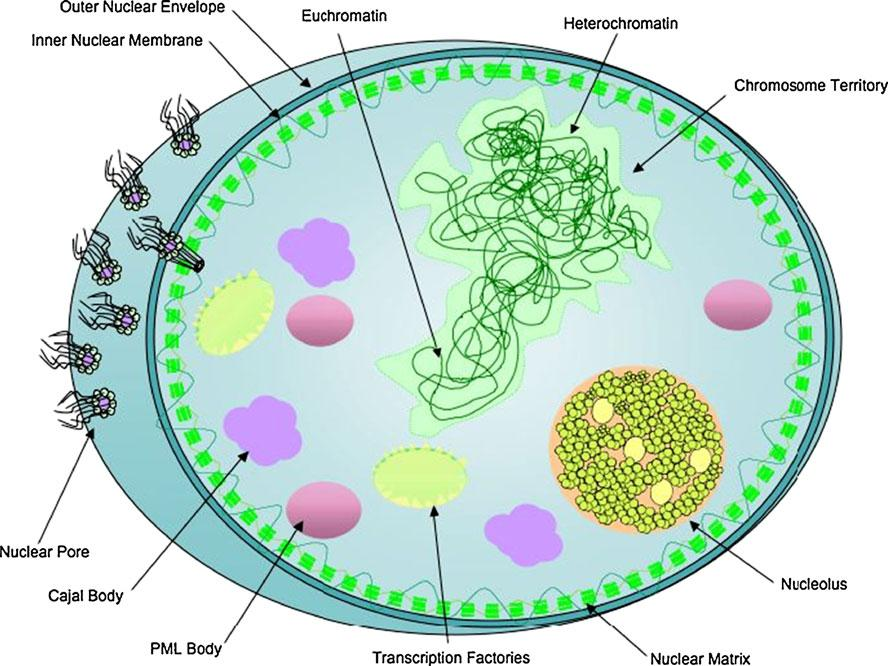
\includegraphics[width=8cm]{nucleus-structure-rynearsonNuclearStructureOrganization2011.jpg}
	\label{fig: nucleus-structure}
	\caption{Estructura y organización nuclear}
	\autocite{rynearsonNuclearStructureOrganization2011}
\end{figure}

\pagebreak

\textbf{Estructura nuclear:}

En el núcleo hay 3 estructuras importantes: la envoltura nuclear, la matriz nuclear y los poros nucleares. La envoltura nuclear, al igual que la membrana plasmática de la célula, está compuesta de una bicapa lipídica de fosfolípidos, la cual separa el citoplasma del contenido del núcleo. Lo que lo diferencia de la membrana plasmática son las proteínas transmembrana y los poros nucleares, que tienen como función seleccionar que entra y que sale del núcleo. Otras funciones de la envoltura nuclear están relacionadas con la organización de la cromatina y la regulación de la expresión genética. También hay una diferencia entre las proteínas transmembrana de la capa externa e interna de la envoltura nuclear, las primeras interactúan con el retículo endoplasmático rugoso (se encuentra cerca de la envoltura nuclear externa) mientras que la segundas solo interactúan directamente con la matriz nuclear.

Por otro lado, la matriz nuclear está compuesta por láminas y proteínas que forman un citoesqueleto dentro de la envoltura nuclear. Por lo tanto, la matriz nuclear existe para proporcionar soporte y estructura al núcleo, dándole un lugar de anclaje al ADN, poros nucleares y proteínas nucleares. Dentro de la matriz nuclear, podemos encontrar una zona llamada espacio intranuclear donde encontramos al genoma. El genoma está organizado en territorios cromosómicos donde encontramos zonas de alta y baja actividad transcripcional, específicamente la eucromatina (ubicada en el centro) y la heterocromatina (ubicada en la periferia). 

\pagebreak

\textbf{Territorios y estructura cromosómica:}

Durante la mitosis,  el genoma condensado se organiza en cromosomas, los cuales se separaran en la división mitótica. Después de la mitosis los cromosomas se desenrollan, formando los territorios cromosómicos. A los territorios cromosómicos que están muy cerca entre ellos, se les llama enquote{vecindario} cromosómico y dentro de este \enquote{vecindario} los territorios cromosómicos interactúan generando una transcripción o translocación genética coordinada. Dentro de los cromosomas también encontramos una distribución (no estricta), donde las bases CG se ubican centralmente mientras que las bases AT se ubican en la periferia.


\begin{figure}[h]
\centering
	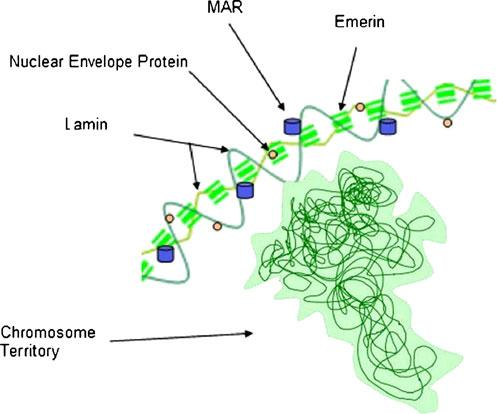
\includegraphics[width=7.5cm]{nucleus-matrix-rynearsonNuclearStructureOrganization2011.jpg}
	\label{fig: nuclear-matrix}
	\caption{Matriz nuclear, incluyendo los lamines y proteínas asociadas}
	\autocite{rynearsonNuclearStructureOrganization2011}
\end{figure}
\newpage

\subsubsection{\texorpdfstring{\citetitle{deyCancerNucleusMorphology2010} (\citeauthor{deyCancerNucleusMorphology2010})}{}}

Hay una gran cantidad de alteraciones morfológicas significativas en el núcleo de las células cancerígenas que pueden ser detectadas por microscopía de luz y con método de tinción. Estas alteraciones suelen estar asociadas a funciones celulares trastornadas de la célula cancerosa. Es por esto que la morfología de los núcleos tiene gran importancia en los estudios, ya que permite comprender los cambios que se producen en el núcleo durante el proceso de carcinogénesis de una manera muy anticipada para así interiorizar en la organización del núcleo del cáncer y ayudar significativamente a entender la patología del núcleo del cáncer y a desarrollar un diagnóstico.


El núcleo de la célula cancerosa muestra muchas características con cambios microscópicos como la alteración de tamaño nuclear, forma, margen, patrón de cromatina, nucleolos, y el espacio perinuclear. De acuerdo con algunos autores, \blockcquote{nickersonNuclearDreamsMalignant1998}{Los cambios progresivos de la estructura nuclear en la malignidad es probable que se asocien con cambios de la matriz nuclear (NM), anormalidades de la membrana nuclear, y la organización de la cromatina nuclear.}


El tamaño en núcleos malignos suele mostrar una variación que es conocida como pleomorfismo. La base de esta variación de tamaño según la teoría del fenotipo de los mutantes se explica en que, si hay inestabilidad genética, esta se produce en el inicio de la carcinogénesis, acá lo que sucede es que las células eligen la mutación óptima para la progresión del cáncer. Por lo tanto, se generan varios subclones de células con esta mutación específica. Es aquí donde estos subclones igual pueden tener relación con los cambios morfológicos variables de las células iniciales, lo que genera una población de células similares con cambios de comportamiento, forma y tamaño que las caracterizan.


Al igual que la forma del núcleo, el margen nuclear cambia en células cancerígenas, estas alteraciones pueden ser vistas como un ranurado nuclear o con convulsiones nucleares. También se ve alterado el engrosamiento del margen el cual aumenta su tamaño a menudo en los núcleos estudiados y esto se debe a la formación de heterocromatina periférica, la cual es una forma de los genes empaquetados en la cromatina de manera más compacta e inactiva. Estas se ubican en la periferia nuclear de las células cancerígenas, por lo que es un buen indicador de un cáncer temprano.


Si bien el núcleo en sí se ve afectado en células cancerígenas también organelos dentro de él se ven alterados y pueden ser de gran ayuda como indicador de un posible cáncer inicial. Uno de estos organelos es el nucleolo el cual tiene como función la biogénesis del ribosoma, esta posee una tasa que depende del metabolismo de la célula. Aquellas células que proliferan adquieren un aumento en la demanda de proteínas, lo que se traduce en un aumento de la tasa de biogénesis ribosomal. De modo que las células que más proliferan tendrán un nucleolo de mayor tamaño que deberá suplir la alta tasa de la biogénesis del ribosoma. Se entiende igual que una célula cancerosa posee una gran tasa de crecimiento por lo tanto se espera que estas tengan nucleolos con un tamaño mayor al normal. Aunque por otro lado según Dey:

\blockcquote[][p. 384]{deyCancerNucleusMorphology2010}{
El agrandamiento nucleolar es por parte de la célula cancerígena, sin embargo, no puede explicarse únicamente por el aumento de la proliferación celular. La neoplasia intraepitelial prostática es un tumor de crecimiento lento, pero muestra grandes y prominentes nucleolos, mientras que la neoplasia intraepitelial cervical es un tumor de rápido crecimiento con nucleolos poco visibles. Esto indica que la tasa de proliferación celular puede no ser el único factor del cambio nucleolar.
}


La matriz nuclear es otro de los distintos indicadores para la detección temprana del cáncer dentro del núcleo o que relaciona al núcleo. Esta matriz nuclear es la estructura de soporte tridimensional del núcleo de la célula que realiza funciones, como determinar la morfología nuclear, la organización del ADN a lo largo del ciclo celular y la estabilización de ADN durante la replicación. Esto le otorga un gran efecto en la morfología del núcleo y como se ha descrito en párrafos anteriores el pleomorfismo está muy ligado a células cancerosas. Por lo tanto, conocer y tener en estudio aquella estructura que se le atribuye la determinación de la morfología nuclear nos da una gran ventaja sobre la detección de células cancerígenas.


También la matriz nuclear contiene una serie de proteínas que llevan el nombre del lugar donde se encuentran (NMP) las cuales según el Pranab son \blockcquote[][p. 386]{deyCancerNucleusMorphology2010}{… específicas en tejidos y enfermedades y por lo tanto son útiles en la detección del cáncer. La detección del NMP22 en la orina en el carcinoma de células transicionales de la vejiga es muy útil en la proyección de los casos recurrentes.} 

\pagebreak

Son estos indicadores los cuales no son todos los que existen, los que a través de su influencia en la morfología del núcleo entregan una significativa ayuda en la detección de células cancerosas en un periodo de tiempo de proliferación corto. 


\begin{figure}[h]
\centering
	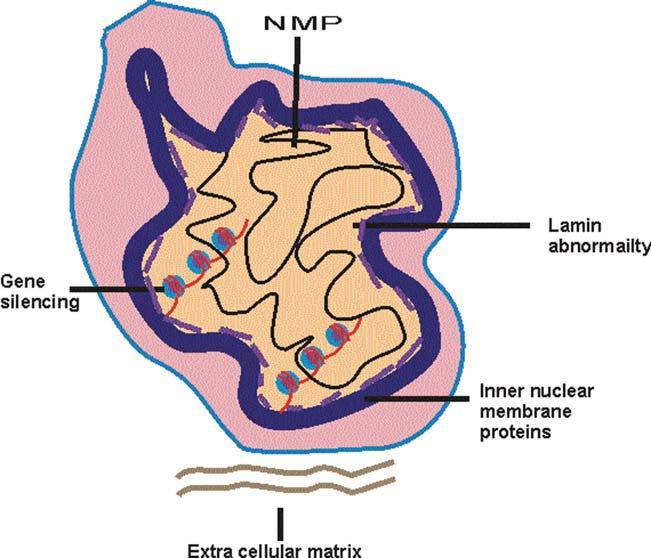
\includegraphics[width=6cm]{nuclear-margin-irregularities-deyCancerNucleusMorphology2010.jpg}
	\label{fig: irregularities-nucleus}
	\caption{Diagrama esquemático muestra los diferentes factores posibles responsables por las irregularidades del margen nuclear}
	\autocite{deyCancerNucleusMorphology2010}
\end{figure}

\newpage

\subsubsection{\texorpdfstring{\citetitle{zinkNuclearStructureCancer2004} (\citeauthor{zinkNuclearStructureCancer2004})}{}}

Entre los cambios morfológicos ya mencionados no tanto en el núcleo en sí, si no que dentro de él, está el que se relaciona con los cromosomas, sus translocaciones y su textura. Estas alteraciones pueden ser tan características de un tipo de cáncer dado y de la etapa en que se utilizan en el diagnóstico del cáncer.


La detección de las translocaciones cromosómicas es un aspecto importante del diagnóstico del cáncer, especialmente en lo que respecta a los cánceres hematológicos, ya que las translocaciones específicas suelen ser características de leucemias o linfomas. Las translocaciones específicas también pueden determinar el pronóstico del paciente. Por ejemplo, Zink explica que:

\blockcquote[][p. 681]{zinkNuclearStructureCancer2004}{
la translocación t(14;18) (q32;q21), que afecta al gen BCL2, se observa en alrededor del 90\% de los linfomas foliculares, que por lo general siguen un curso indolente. Por el contrario, la translocación t(11;14) (q13;q32) es una característica del linfoma de células del manto, que es una enfermedad de rápida progresión.
}


También es importante diagnosticar los cambios en la textura de la cromatina, que se observan con frecuencia en las células cancerosas. Estos son probablemente causados por la condensación y descondensación de los dominios de cada cromatina. De acuerdo con algunos autores, \blockcquote{lukasovaTopographyGeneticLoci2004}{las diferencias en el grado de condensación de la cromatina y en la organización de la cromatina de las células normales y tumorales también están indicadas por las diferentes distancias entre los loci de los genes.
}

\pagebreak

Dos configuraciones de cromatina fácilmente observables con importancia diagnóstica son el \enquote{engrosamiento de la cromatina} y la \enquote{cromatina abierta} exagerada, que corresponden a un aumento o a una pérdida de agregados de heterocromatina, respectivamente. El engrosamiento de la cromatina es poco común en las células normales y da lugar a mayores agregados de heterocromatina. Puede ser inducido en diferentes tipos de células por la expresión de HRAS activada. El grado de engrosamiento de la cromatina no está relacionado con la fracción de células que proliferan en las líneas celulares, pero se correlaciona estrechamente con el potencial metastásico. De este modo se puede estudiar el engrosamiento de la cromatina como motivo para una posible metástasis.


\begin{figure}[h]
\centering
	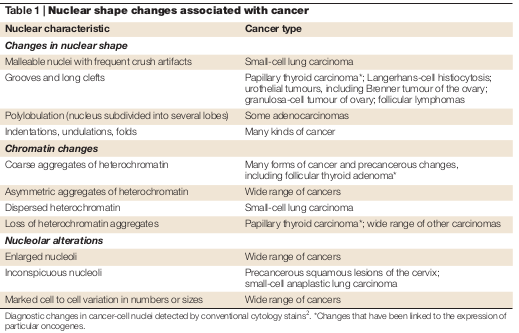
\includegraphics[width=7.5cm]{table-1-zinkNuclearStructureCancer2004.png}
	\label{fig: zink-table-1}
	\caption{Cambios en nucleos afectados}
	\autocite{zinkNuclearStructureCancer2004}
\end{figure}
\newpage

\subsubsection{\texorpdfstring{\citetitle{thermanStructureOriginGiant1983} (\citeauthor{thermanStructureOriginGiant1983})}{}}

El ciclo nuclear normalmente posee una alternancia entre replicación cromosómica y mitosis, que, en caso de alterarse, puede producir diversas modificaciones en la mitosis y por ende anormalidades cromosómicas características de cáncer. Esto puede traer poliploidía en los núcleos debido a diversas razones ligadas a la mitosis, como la supresión del huso. Esto se ha estudiado bastamente en invertebrados, plantas y protistas, pero en mamíferos la información estudiada solo se reduce a modificaciones mitóticas en tumores malignos. En la mayoría de los cánceres existen los llamados núcleos gigantes, pero es importante señalar, que las llamadas modificaciones mitóticas comunes en el cáncer también se han encontrado en células normales.


En este estudio se eligieron dos carcinomas invasivos de células en el cuello uterino, ya que eran prominentes para un estudio detallado. En los tumores los nucleos iban de pequeños a grandes, donde los grandes no se pudieron dividir. Los nucleos variaron de estar teñidos de manera uniforme a tener cromocentros prominentes. Ninguna celula de los tumores mostró cromatina X identificable (esta cromatina es naturalmente imposible de determinar en núcleos con cromatina prominente). Los dos tumores tenían núcleos gigantes, pero eran diferentes en varios aspectos. En el caso 1 casi todos los núcleos presentaban comocentros prominentes donde parece ocurrir principalmente la endomitosis (por ende poliploidía).


\begin{figure}[h]
\centering
	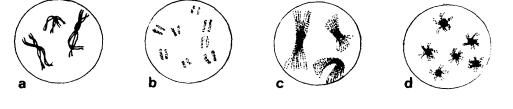
\includegraphics[width=12cm]{endopolyploid-nuclei-thermanStructureOriginGiant1983.jpg}
	\label{fig: endopolyploid-nuclei}
	\caption{Diagrama de diferentes tipos de endopolyploid nuclei: (a) profase con diplocromosomas, (b) endometafase-endoanafase, (c) núcleo con cromosomas politénicos, (d) núcleo con cromocentros grandes}
	\autocite{thermanStructureOriginGiant1983}
\end{figure}

\pagebreak

\begin{figure}[h]
\centering
	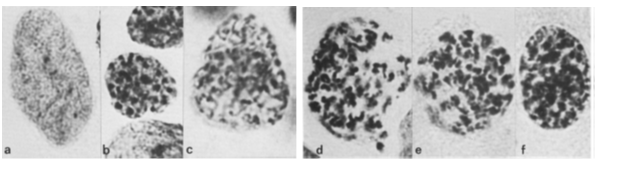
\includegraphics[width=10cm]{cancerous-nuclei-thermanStructureOriginGiant1983.png}
	\label{fig: cancerous-nuclei}
	\caption{Diagrama de núcleos cancerosos: (a) núcleo sin cromocentros o cromatina X, (b) núcleo con cromocentros, (c) profase normal, (d) probable endoprofase, (e, f) endometafase-endoanafase (caso 1). x 3000}
	\autocite{thermanStructureOriginGiant1983}
\end{figure}

\pagebreak

\subsubsection{\texorpdfstring{\citetitle{madrazoCellIntegrinsNew2017} (\citeauthor{madrazoCellIntegrinsNew2017})}{}}

El núcleo separa y contiene el genoma del citoplasma, las células cancerígenas presentan una morfología nuclear aberrante, ya sea en forma y volumen, con regiones de cromatina aberrantes. A pesar de eso estos defectos en los componentes nucleares, no son conductores al desarrollo del cáncer, pero sí una consecuencia de la evolución de este. Las células cancerosas manifiestan muchas anomalías epigenéticas, que conducen a inestabilidad genómica y expresión génica aberrante durante la progresión y la recurrencia del cáncer. Debido a la arquitectura nuclear aberrante de las células cancerosas, los cambios nucleares se han propuesto como un sello distintivo del cáncer y pueden conducir a la identificación de nuevos desarrollos terapéuticos.


Las integrinas son proteínas receptoras transmembrana del tipo 1, poseen un dominio extracelular, una región transmembrana y una cola citoplasmática, se encuentran presentes en diversos procesos desempeñando un papel fundamental. Debido a estas mismas funciones es que se ven implicadas en diversas patologías, entre ellas el cáncer. Así, la mediación de integrinas pareciera impulsar la proliferación de células cancerígenas y metástasis. De esta forma las células  cancerígenas utilizan las integrinas para regular la señalización del factor de crecimiento o en otros casos ayuda a mantener la población del cáncer estableciendo una relación entre las integrinas y el recién mencionado. Para las células cancerosas, se ha demostrado que las integrinas y sus glicoproteínas asociadas apoyan la adhesión de las células cancerosas y contribuyen a la progresión tumoral y a los fenotipos de cáncer invasivo. Es ampliamente conocido que las integrinas son críticas para la migración de células cancerosas en espacios confinados. La regulación de la forma, posición y deformación nuclear es fundamental para controlar la migración de células tanto normales como cancerosas.


La deformabilidad nuclear es fundamental para permitir la migración de células cancerosas en condiciones confinadas . Durante la migración celular, el núcleo se vuelve más maleable y sensible a las fuerzas aplicadas desde el citoesqueleto. Múltiples componentes nucleares determinan la deformabilidad nuclear, incluidas las láminas, la cromatina y el nucleoplasma.


\newpage


\subsection{Análisis Aplicación de Machine Learning}


\subsubsection{\texorpdfstring{\citetitle{kourouMachineLearningApplications2015} (\citeauthor{kourouMachineLearningApplications2015})}{}}

Dentro de machine learning tenemos dos fases principales, la estimación de dependencias desconocidas en un sistema, y el uso de estas estimaciones para producir outputs nuevos dado inputs desconocidos. Para realizar estos procesos, tenemos dos tipos principales de algoritmos, supervisado y no supervisado. En el proceso supervisado, uno entrega información con un output conocido. Un ejemplo de esto podría ser, las medidas de un tumor como input y el potencial de crecer como output. En el no supervisado, uno solo entrega información sin saber su output. Por lo cual el algoritmo sólo puede encontrar patrones o grupos dentro de la información dada.

\noindent
Un ejemplo de clasificación lo podríamos ver en este gráfico:

\begin{figure}[h]
\centering
	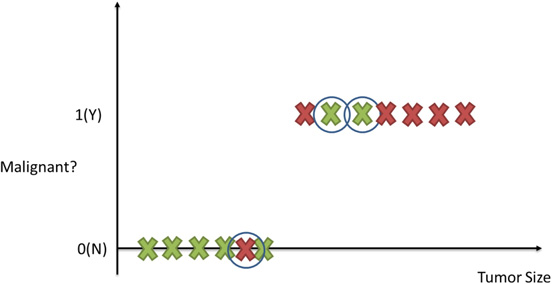
\includegraphics[width=11cm]{1d-classification-kourouMachineLearningApplications2015.png}
	\label{fig: 1d-classification}
	\caption{Grafico relacionando el tamaño de un tumor con el estado de malignidad del tumor}
	\autocite{kourouMachineLearningApplications2015}
\end{figure}

Donde podríamos aplicar un algoritmo, para encontrar una línea que separe nuestros datos conocidos. Y de esa forma, cuando tengamos nuevos datos, podemos automáticamente clasificar.

\pagebreak

\noindent
Donde podríamos llegar a:

\begin{figure}[h]
\centering
	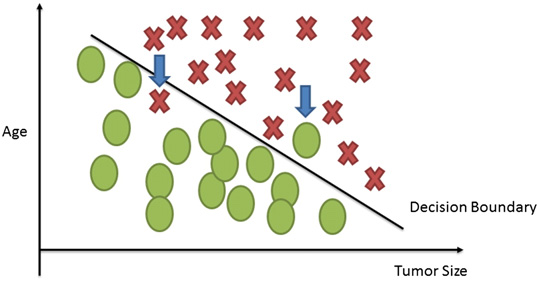
\includegraphics[width=9cm]{2d-classification-kourouMachineLearningApplications2015.png}
	\label{fig: 2d-classification}
	\caption{Grafico relacionando el tamaño de un tumor y edad del paciente con el estado de malignidad del tumor}
	\autocite{kourouMachineLearningApplications2015}
\end{figure}


Donde ahora estamos trabajando con 2 fuentes de información, tamaño y edad. Por lo cual podemos ver que este método lo podemos generalizar fácilmente a diferentes dimensiones.

Otro método más reciente es denominado \enquote{ANN} y consiste de una \enquote{caja-negra} donde nosotros no sabemos como llega al resultado. Este método es muy parecido a como nosotros pensamos, ya que está modelado desde cómo funcionan las neuronas. Consiste en capas de nodos unidos por conexiones arbitrarias entre ellas. 

\begin{figure}[h]
\centering
	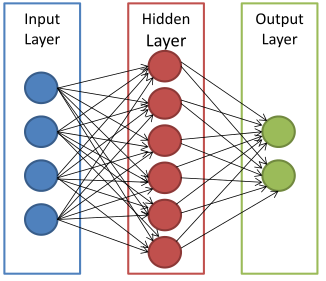
\includegraphics[width=8cm]{ann-kourouMachineLearningApplications2015.png}
	\label{fig: ann-classification}
	\caption{Grafico de un estructura general de un ANN}
	\autocite{kourouMachineLearningApplications2015}
\end{figure}

\pagebreak

Finalmente, tenemos el algoritmo de árbol, el cual funciona en clasificar nuestra información por cada dimensión que le damos. De forma que, por ejemplo, aprende a reconocer que si tienes cierta edad y, al mismo tiempo, tienes una deformación de tu núcleo, puede predecir que tienes un cáncer peligroso.

\begin{figure}[h]
\centering
	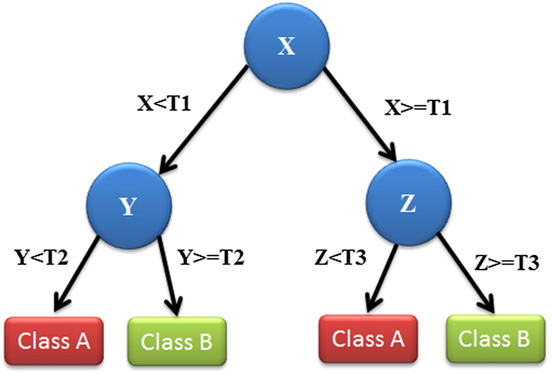
\includegraphics[width=8cm]{tree-kourouMachineLearningApplications2015.png}
	\label{fig: tree-classification}
	\caption{Grafico de un estructura general de un Arbol}
	\autocite{kourouMachineLearningApplications2015}
\end{figure}

\newpage

\subsubsection{\texorpdfstring{\citetitle{sirinukunwattanaLocalitySensitiveDeep2016} (\citeauthor{sirinukunwattanaLocalitySensitiveDeep2016})}{}}

En el uso de machine learning para cualquier tipo de aplicación, lo más importante es la data que nosotros le entregamos a nuestro modelo. Por lo que, en su uso en detección de cáncer por medio de irregularidades nucleares, vamos a tener dos problemas. La calidad de nuestros núcleos segmentados y la cantidad que podemos procesar. Este paper nos entrega un método nueva de como usar machine learning para habilitar la detección y segmentación automática de estos núcleos. 


\begin{figure}[h]
\centering
	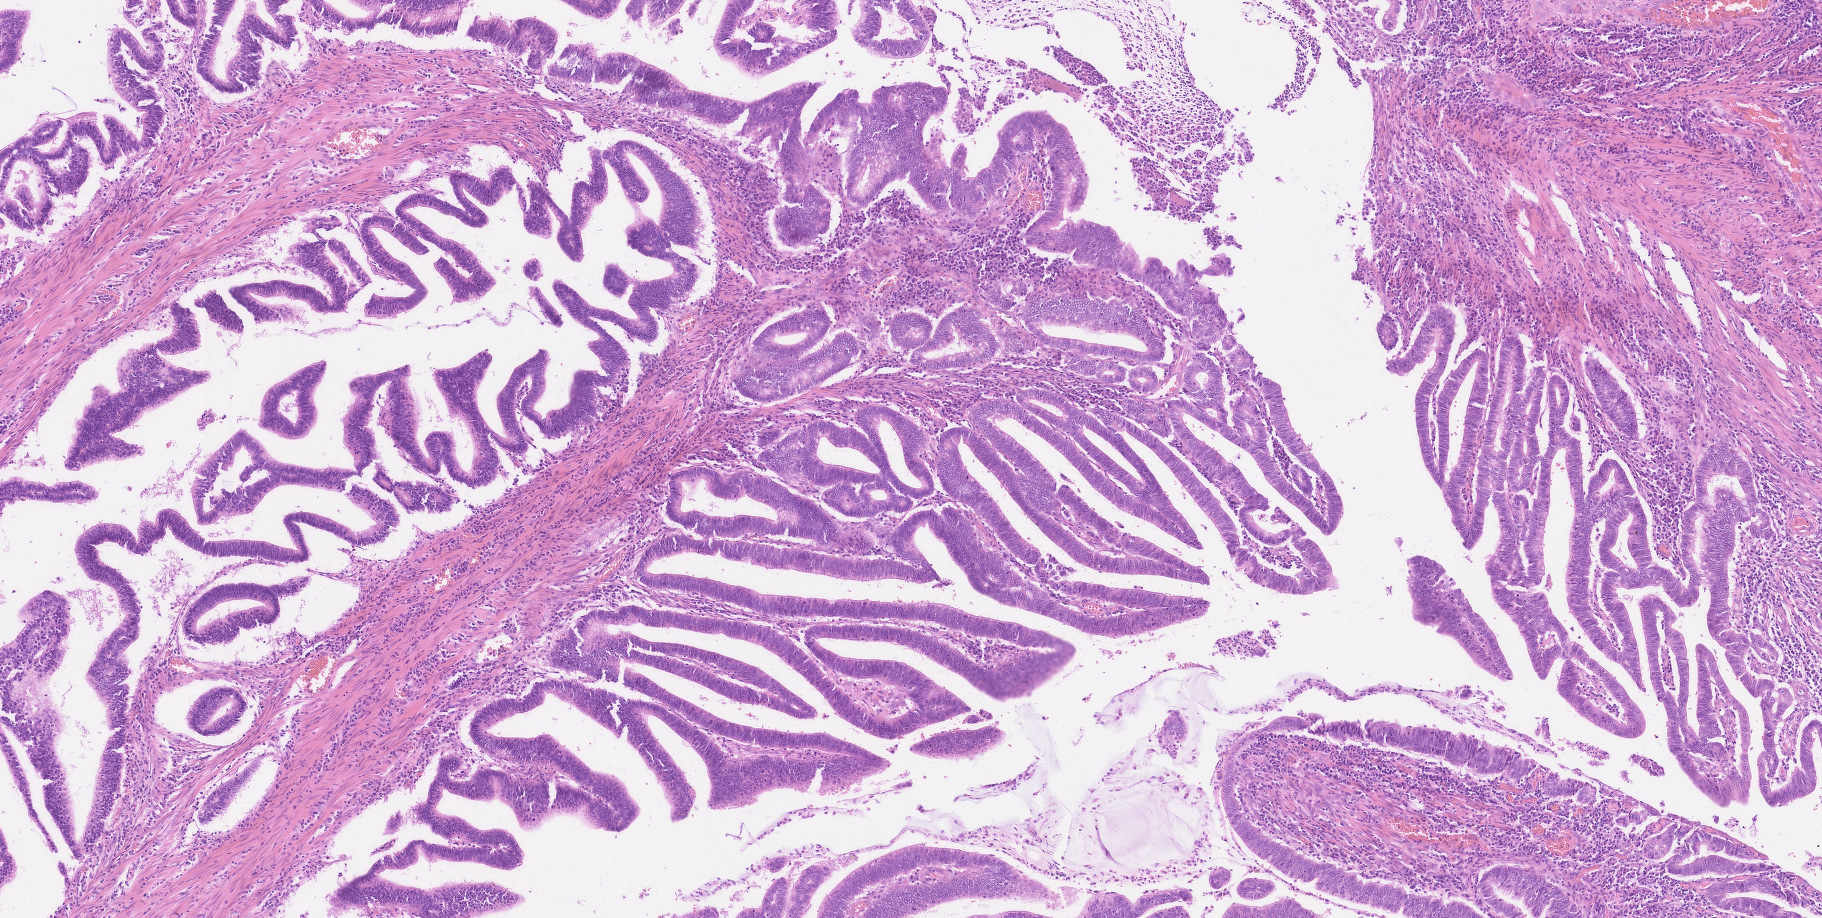
\includegraphics[width=8cm]{hm-stain-sirinukunwattanaLocalitySensitiveDeep2016.png}
	\caption{Foto H\&E}
	\autocite{kourouMachineLearningApplications2015}
	\label{fig: hm-stain}
\end{figure}

Para esto usamos un modelo CNN que es un modelo derivado del ANN visto en el paper \autocite{kourouMachineLearningApplications2015}. Este modelo es capaz de tomar nuestras imágenes H\&E (hematoxylin and eosin), e.j. \cref{fig: hm-stain}, y aprender donde están los núcleos. Esto se realizó con 100 imágenes H\&E de 500 x 500 píxeles. Donde expertos y estudiantes clasificaron manualmente los núcleos presentes en cada imagen. Donde, en total, se anotaron más de 20 000 núcleos individuales.

\begin{figure}[h]
	\begin{subfigure}{.3\textwidth}
		\centering
		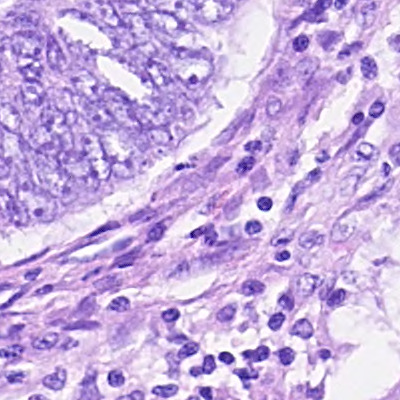
\includegraphics[width=4cm]{a-sirinukunwattanaLocalitySensitiveDeep2016.png}
		\caption{Input}
	\end{subfigure}
	\begin{subfigure}{.3\textwidth}
		\centering
		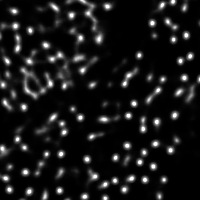
\includegraphics[width=4cm]{b-sirinukunwattanaLocalitySensitiveDeep2016.png}
		\caption{Mascara}
	\end{subfigure}
	\begin{subfigure}{.3\textwidth}
		\centering
		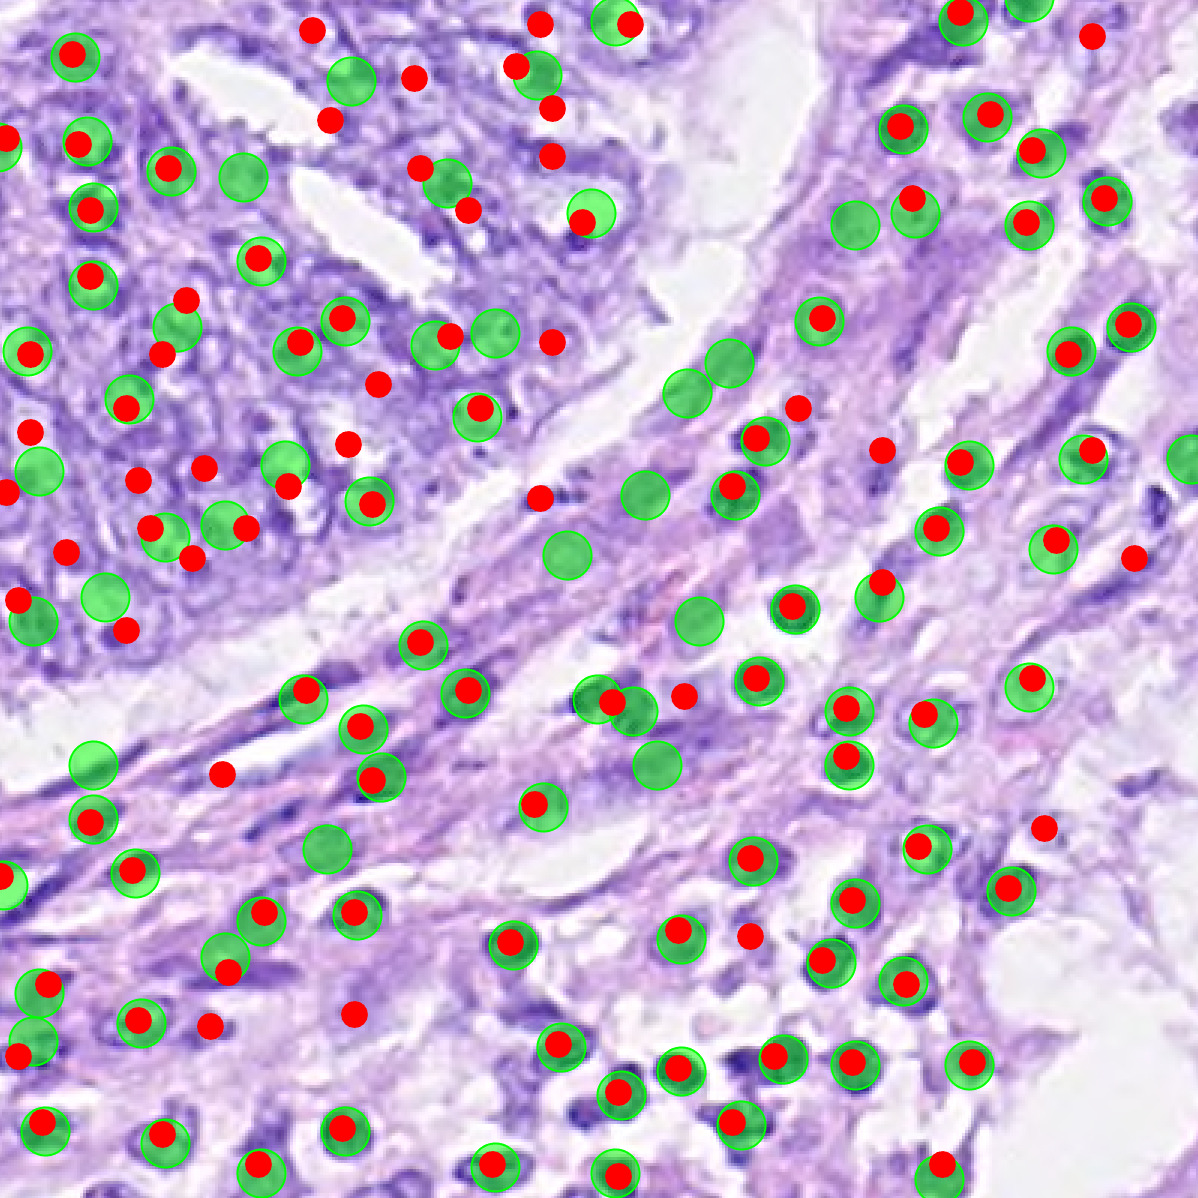
\includegraphics[width=4cm]{c-sirinukunwattanaLocalitySensitiveDeep2016.png}
		\caption{Núcleos marcados}
	\end{subfigure}
\end{figure}

Usando el método descrito anteriormente, se logró llegar a una precisión de 0.781, lo cual significa que de cada 1000 puntos clasificadas, 781 eran verdaderamente núcleos. También se logró llegar a un recall de 0.827, lo cual significa que de cada 1000 núcleos presentes, se clasificaron 827. Esto es relevante ya que algoritmos pasados tenían precisión y recall en los alrededores de 0.600 cada uno. Por lo que las estadísticas obtenidas son una mejora.

Con este algoritmo se demuestra que es posible clasificar núcleos de células automáticamente. Lo que nos dice, que entrenar un modelo que usó características de estos núcleos no sería muy costoso. Por lo que, no habilita el uso de muchos algoritmos, los cuales, algunos, serán mencionados más abajo.


\newpage

\subsubsection{\texorpdfstring{\citetitle{kancherlaEarlyLungCancer2013} (\citeauthor{kancherlaEarlyLungCancer2013})}{}}

Actualmente uno de los pilares más importantes a la hora de combatir al cáncer, es la detección temprana y análisis correcto del tipo de cáncer, detección de metástasis, características del microambiente tumoral, etc. Para lograr esto de la forma más eficiente y rápida, se han usado un sin fin de nuevas tecnologías, pero la que ha dado mejores resultados hasta ahora, es el uso de machine learning. 

El cáncer de pulmón es el cáncer que genera más muertes \autocite{CommonCancerTypes2015b}, por lo que ha atraído mucho atención. También se debe mencionar que se busca la detección temprana del cáncer, ya que esto sube de manera significativa la posibilidades de sobrevivencia del paciente \autocite{WHOEarlyDetection}.  En este estudio se utilizaron las características del núcleo (de células tumorales) para crear un algoritmo de machine learning que logre realizar un detección temprana del cáncer de pulmón. 

Para llevar a cabo esta investigación se hizo un experimento con muestras de esputo (secreciones provenientes del bronquios) de 15 pacientes diagnosticados recientemente con cáncer pulmonar y 13 pacientes normales pero que eran fumadores empedernidos (un paquete de cigarros al dia).  Para observar las muestra se utilizó un etiquetado de TCPP (fluorescente), que aumentó el crecimiento de lipoproteínas particulares del revestimiento de la superficie de células cancerígenas, por lo que luego se utilizó un microscopio ultravioleta (con un filtro FITC) para observar las células de las muestras de esputo. Luego se utilizaron técnicas de procesamiento de imágenes (de las muestras antes mencionadas) para separar y obtener células individuales, y de estas obtener características que sirvan en la detección de cáncer. Las característica iniciales que se obtuvieron fueron: intensidad/color, forma y textura. El set inicial contenía en total 71 características pero luego de una optimización y uso de métodos capaces de identificar un set con mayor precisión, se obtuvieron 79 características. Para el uso de técnicas de machine learning se utilizó este set de características modificado (79 características) y un conjunto de datos con 60 muestras de cáncer y 59 con muestras normales (119 puntos de data en total). Los resultados finales entregaron una precisión de 87\% con lo que se concluyó que los métodos de machine learning basados en el núcleo poseen un gran potencial y eficacia (comparado con los demás métodos existentes) en la detección temprana de cáncer, permitiendo mejorar el monitoreo del tratamiento, detección de recurrencia de cáncer pulmonar e identificación de pacientes que necesiten un procedimiento de diagnóstico invasivo.


\newpage

\subsubsection{\texorpdfstring{\citetitle{wangPredictionRecurrenceEarly2017} (\citeauthor{wangPredictionRecurrenceEarly2017})}{}}

Por el paper \autocite{kancherlaEarlyLungCancer2013}, podemos ver que es factible usar machine learning para detectar el cáncer de manera precisa y temprana. En este estudio, el cual fue realizado en Estados Unidos, se analiza la recurrencia del cáncer de pulmón. Se utilizaron las imágenes patológicas que se obtuvieron luego de hacerles un examen radiográfico a pacientes, a los cuales ya se les había removido un cáncer de pulmón. Con estas imágenes se utilizó un algoritmo de deep learning capaz de identificar y detectar las características principales que tiene un cáncer de recurrencia.

Este algoritmo utilizó 15 \enquote{features}, lo cual significa que se le entregó 15 puntos de información por paciente. Estos puntos de información se pueden separar en 3 categorías principales:

\begin{itemize}
	\item Forma del núcleo
	\item Orientación del núcleo
	\item Textura del núcleo
\end{itemize}

Con esto, el algoritmo se encargó de poder clasificar a los pacientes en dos grupos principales. Los de no recurrencia y los de recurrencia. Para esto, se tomó el grupo colectivo de paciente y se separaron en 3 grupos. El primer grupo se usó para entrenar el algoritmo y los otros dos se usaron para revisar \enquote{accuracy} del algoritmo.

En conclusión, el estudio pudo llegar a una exactitud de 82\% lo cual significa, que de cada 100 imágenes, se clasificaron 82 de manera correcta. Dado que estas imágenes se deben tomar independientemente de si se utilizan para algún tipo de algoritmo, ya que se necesitan para que los médicos revisen visualmente al paciente , se esta efectivamente aprovechando el trabajo ya hecho. Por lo que predecir con el algoritmo, que tiene un 82\% de exactitud, quién va a tener una recurrencia va a ser de mucha ayuda para los médicos y pacientes.


\newpage

\printbibliography

\end{document}